\begin{homeworkProblem}
\textbf{A plane wave (E-field Perpendicular to plane of incidence) is incident from air ($n=1$) at angle
of incidence $\theta_i$.}

\begin{homeworkSection}{a}
\textbf{Using boundary condition at the interface, derive the formula for Reflectivity in this case
(equation 7.41).}
\\

This exact problem is solved in any electrodynamics text. The approach here is borrowed heavily from John Jackson's Electrodynamics. I refer the interested reader to Section 7.3 of this text.

To solve this problem I must first establish the boundary conditions on the electric and magnetic fields of the plane wave. For an electromagnetic wave of complex magnitude $E_0$ incident on an interface at an angle $\theta_i$ it will reflect with amplitude $E_0^{''}$ and transmit with amplitude $E_0^{'}$. Maxwell's equations impose the following four boundary conditions on the $E$ field (the boundary conditions on the magnetic field have been imposed on the $E$ field by the relationship between $E$ and $B$ for a plane wave):
\begin{align*}
   \big[ \epsilon (E_0 + E_0'')- \epsilon'E_0' \big]  \cdot \hat{n} &= 0 \\
   \big[\vec{k}\times E_0 +\vec{k''}\times E_0'-\vec{k'}\times E_0''\big]\cdot \hat{n} &= 0 \\
   \big(E_0 + E_0'' - E_0'\big)\times \hat{n} &= 0 \\ 
   \big[ \frac{1}{\mu}(\vec{k}\times E_0 + \vec{k''}\times E_0'') - \frac{1}{\mu'}(\vec{k'} \times E_0') \big] \times \hat{n} &= 0
\end{align*}

For an E-field with its polarization perpendicular to the plane of incidence the third and fourth relationships yield:
\begin{align*}
   E_0 + E_0''-E_0' &= 0 \\
   \sqrt{\frac{\epsilon}{\mu}}(E_0 - E_0'')\cos\theta_i - \sqrt{\frac{\epsilon'}{\mu'}}E_0'\cos\theta_r & = 0
\end{align*}
Above are two equations with three unknowns. Identifying $\frac{E_0'}{E_0}$ as one variable and $\frac{E_0''}{E_0}$ as another variable we can see that these two equations only involve these two variables. Next, we can utilize our skills in algebraic arithmetic to yield the following expressions:

  \begin{problemAnswer}{
\frac{E_0'}{E_0} &= \frac{2 n \cos\theta_i}{n\cos\theta_i + \frac{\mu}{\mu'}\sqrt{n'^2-n^2\sin^2\theta_i}} \\
  \frac{E_0''}{E_0} &= \frac{n\cos\theta_i - \frac{\mu}{\mu'}\sqrt{n'^2-n^2\sin\theta_i}}{n\cos\theta_i+\frac{\mu}{\mu'}\sqrt{n'^2-n^2\sin^2\theta_i}}}
\end{problemAnswer}

\end{homeworkSection}
\begin{homeworkSection}{b}
\textbf{In the case of grazing incidence $\theta_I \approx \frac{\pi}{2}$ on a dielectric medium whose index of refraction is $n = 1-\delta$ (where $\delta << 1$) so is almost unity. This is the case for most materials in the x-ray regime. Use $\phi_I = \frac{\pi}{2} - \theta_I$ show that the critical angle is $\phi_c \approx \sqrt{2\delta}$. (this is the angle for which the refracted angle is $\frac{\pi}{2}$)}
\\

The critical angle is the angle at which $\sin(\theta_2)= \pi/2$ in Snell's law - $n_1 \sin\theta_1 = n_2\sin\theta_2$. If $n_1$ is air (which it is claimed to be in this problem) then the critical angle is related to the incident angle $\theta_I$ through $\sin\theta_I = n_2$. Since $\theta_I \approx \pi/2$ $\sin\theta_I = \sin(\pi/2-\phi_I) = \cos(\phi_I)$. Now, $\phi_I$ is pretty small according to the problem statement. Thus, $1+\phi_I^2/2 \approx n_2 = 1-\delta$ and, trivially, 
\begin{problemAnswer}{
  \sqrt{2\delta}\approx \phi_I}
\end{problemAnswer}
\end{homeworkSection}

\begin{homeworkSection}{c}
\textbf{Continuing with the case outlined in part b, derive the reflectivity $R_\bot \approx \frac{|\phi_I-\sqrt{\phi_I^2-\phi_c^2}|^2}{|\phi_I+\sqrt{\phi_I^2-\phi_c^2}|^2}$}
\\

To derive the reflectivity $R_\bot$ I need to consider the expression $\frac{n\cos\theta_i - \frac{\mu}{\mu'}\sqrt{n'^2-n^2\sin^2\theta_i}}{n\cos\theta_i+\frac{\mu}{\mu'}\sqrt{n'^2-n^2\sin^2\theta_i}}$ which relates the amplitude of the incident wave of that to the reflected wave. Now, consider that $\theta_i = \pi/2 - \epsilon$ where $\epsilon << 1 $. So, $\cos\theta_i = \sin\phi_i \approx \phi_i$. Furthermore:
\begin{align*}
\sqrt{n'^2-\sin^2\theta_i} &= \sqrt{(1-\delta)^2-\sin^2\theta_i} \\
& = \sqrt{\cos^2\theta_i - 2\delta} \\
& \approx \sqrt{\phi_i^2-2\delta} \\
& \approx \sqrt{\phi_i^2-\phi^2_c}
\end{align*}

The final step before expressing the final answer is to realize that for optical (and above) frequencies it is typical for most materials that $\mu = \mu'$. That is, most materials have the same permeability as vacuum. These results contract the expression for the reflected amplitude to: 
\\

\begin{problemAnswer}
{
R_\bot = \frac{\phi_i - \sqrt{\phi_i^2 - \phi_c^2}}{\phi_i+\sqrt{\phi_i^2-\phi_c^2}}
}
\end{problemAnswer}
\end{homeworkSection}
\begin{homeworkSection}{d}
\textbf{Plot $R_\bot$ vs $\frac{\phi_i}{\phi_c}$ with $\frac{\phi_I}{\phi_c}$ ranging from 0 to 3.}
\\

The plot is included in Figure 3.

\begin{figure}
\centering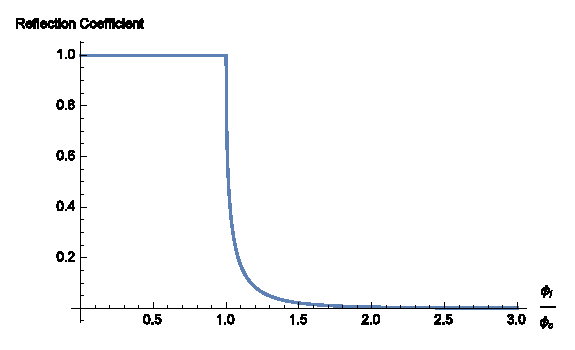
\includegraphics[width=.5\linewidth]{Images/RefCoefProb4.eps}
\caption{Reflection coefficient plotted for $\frac{\theta_i}{\theta_c} = 0 \rightarrow 3$}
\end{figure}
\end{homeworkSection}
\end{homeworkProblem}
